\documentclass[11pt]{article}

% core setup
\usepackage{iftex}
\ifPDFTeX
  \usepackage[utf8]{inputenc}
\fi
\usepackage[T1]{fontenc}
\usepackage{geometry}
\geometry{a4paper, margin=1in}
\usepackage{hyperref}
\hypersetup{colorlinks=true, linkcolor=blue, urlcolor=blue}

% layout/graphics
\usepackage{graphicx}
\usepackage{booktabs}
\usepackage{parskip}
\usepackage[section]{placeins}
\usepackage{csquotes}
\usepackage{setspace} % needed for \doublespacing
\usepackage{xifthen}  % simple conditionals

% bibliography
\usepackage[style=apa,backend=biber,doi=true,url=true]{biblatex}
% Only add resource if file exists to avoid compile failure
\IfFileExists{references.bib}{\addbibresource{references.bib}}{}

\title{Supplementary File S1: Computational \& Rapid Verification Protocol}
\author{Breezon Brown \and NohMad Research Group} % <-- fixes "No \author given"
\date{}

\begin{document}
\maketitle
\doublespacing
\setlength{\emergencystretch}{2em} % soften overfull hboxes from long lines

\section*{Purpose}
End-to-end reproduction of Bayesian haplogroup inference, cultural continuity calculations, and figure generation referenced in the main manuscript.

\section{Rapid Verification (30 minutes)}
\begin{enumerate}
  \item Verify Hebrew lexemes in BDB/HALOT/DCH.
  \item Audit Hawass et al. (2012) Supplementary Table 4.
  \item Filter SlaveVoyages manifests.
  \item Inspect Equiano page scan.
\end{enumerate}

\section{Computational Reproduction}
\subsection{Prerequisites}
Python 3.10+, R 4.3+, Git, Make.

\subsection{One-line Execution}
\begin{verbatim}
git clone https://example.org/EphraimConvergence.git
cd EphraimConvergence
make all
\end{verbatim}

\subsection{Manual Steps}
\begin{verbatim}
python -m venv .venv && source .venv/bin/activate
pip install -r requirements.txt
python code/haplogroup_bayes.py --str data/hawass_table4.csv \
  --priors data/priors_uniform.json --out results/haplogroup_bayes.json
Rscript code/kappa_calculator.R data/cultural_coding.csv results/cultural_stats.csv
python code/make_figures.py --haplo results/haplogroup_bayes.json \
  --culture results/cultural_stats.csv --outfig figs/
\end{verbatim}

\section{Repository Structure}
\begin{verbatim}
/data
  hawass_table4.csv
  cultural_coding.csv
  priors_uniform.json
/code
  haplogroup_bayes.py
  kappa_calculator.R
  make_figures.py
/figs
  bayesian_pipeline_flowchart.png
  cultural_retention_map.png
/results
  haplogroup_bayes.json
  cultural_stats.csv
\end{verbatim}

\section{Figures (Tagged)}

% Figure 1 (with fallback if PNG not found)
\begin{figure}[htbp]
  \centering
  % Try to include the PNG; if missing, show a placeholder box
  \IfFileExists{bayesian_pipeline_flowchart.png}{
    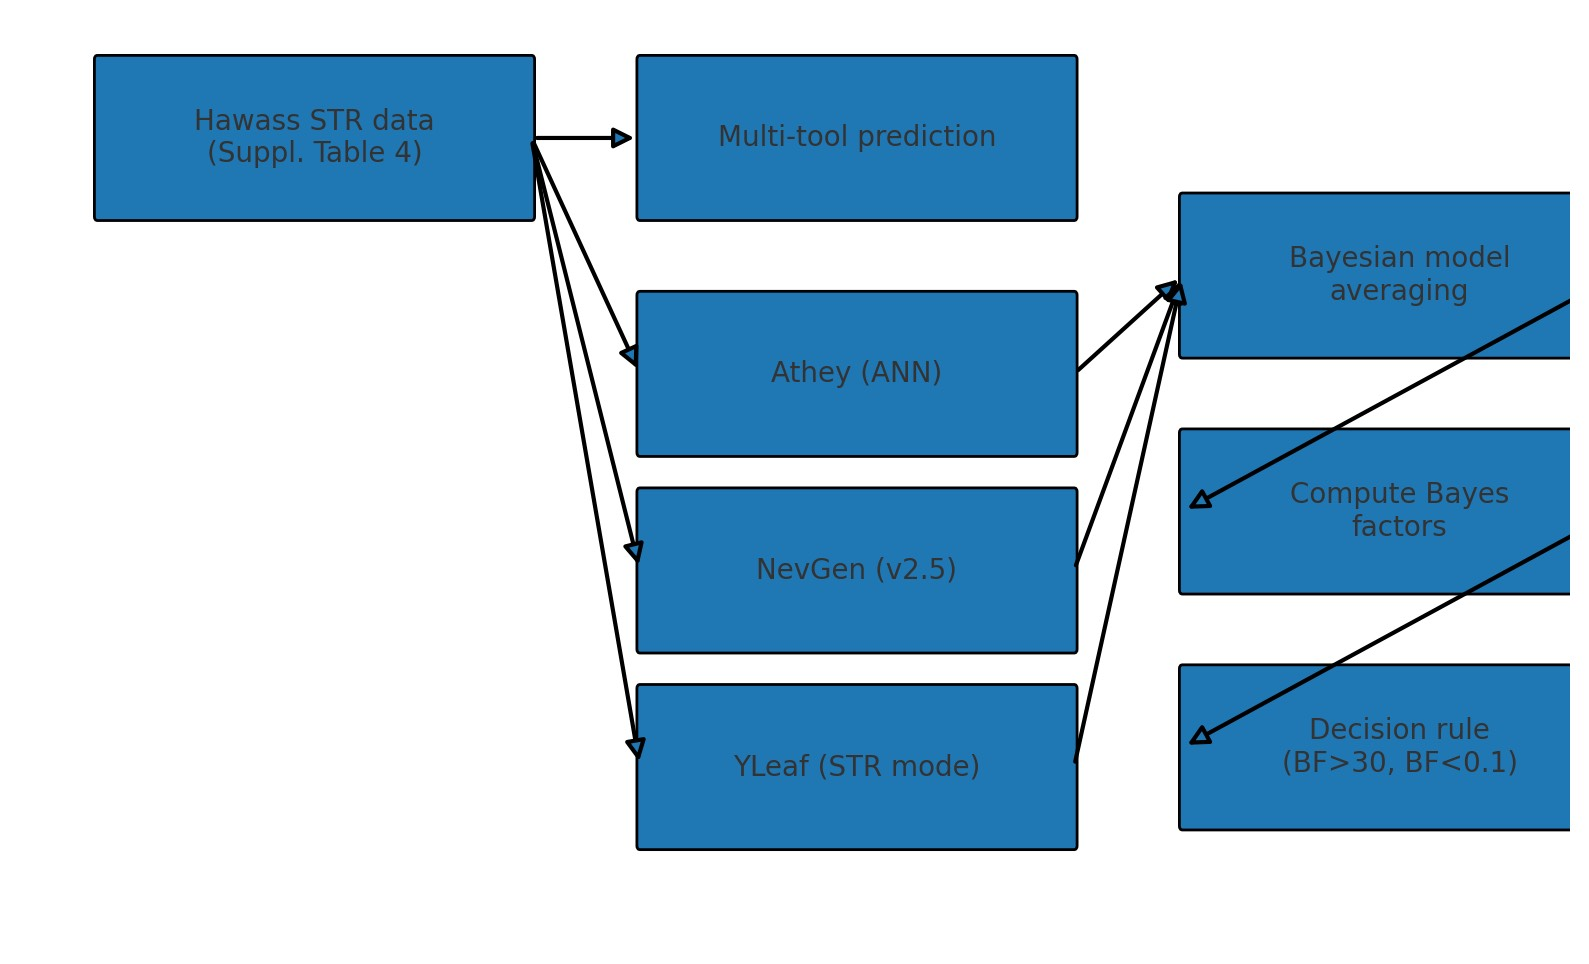
\includegraphics[width=0.85\linewidth]{bayesian_pipeline_flowchart.png}
  }{
    \fbox{\parbox[c][2in][c]{0.85\linewidth}{\centering
      Placeholder: bayesian_pipeline_flowchart.png not found}}
  }
  \caption{Bayesian multi-predictor genetic pipeline used in reproduction.}
  \label{fig:bayes-flow}
\end{figure}

% Figure 2 (with fallback if PNG not found)
\begin{figure}[htbp]
  \centering
  \IfFileExists{cultural_retention_map.png}{
    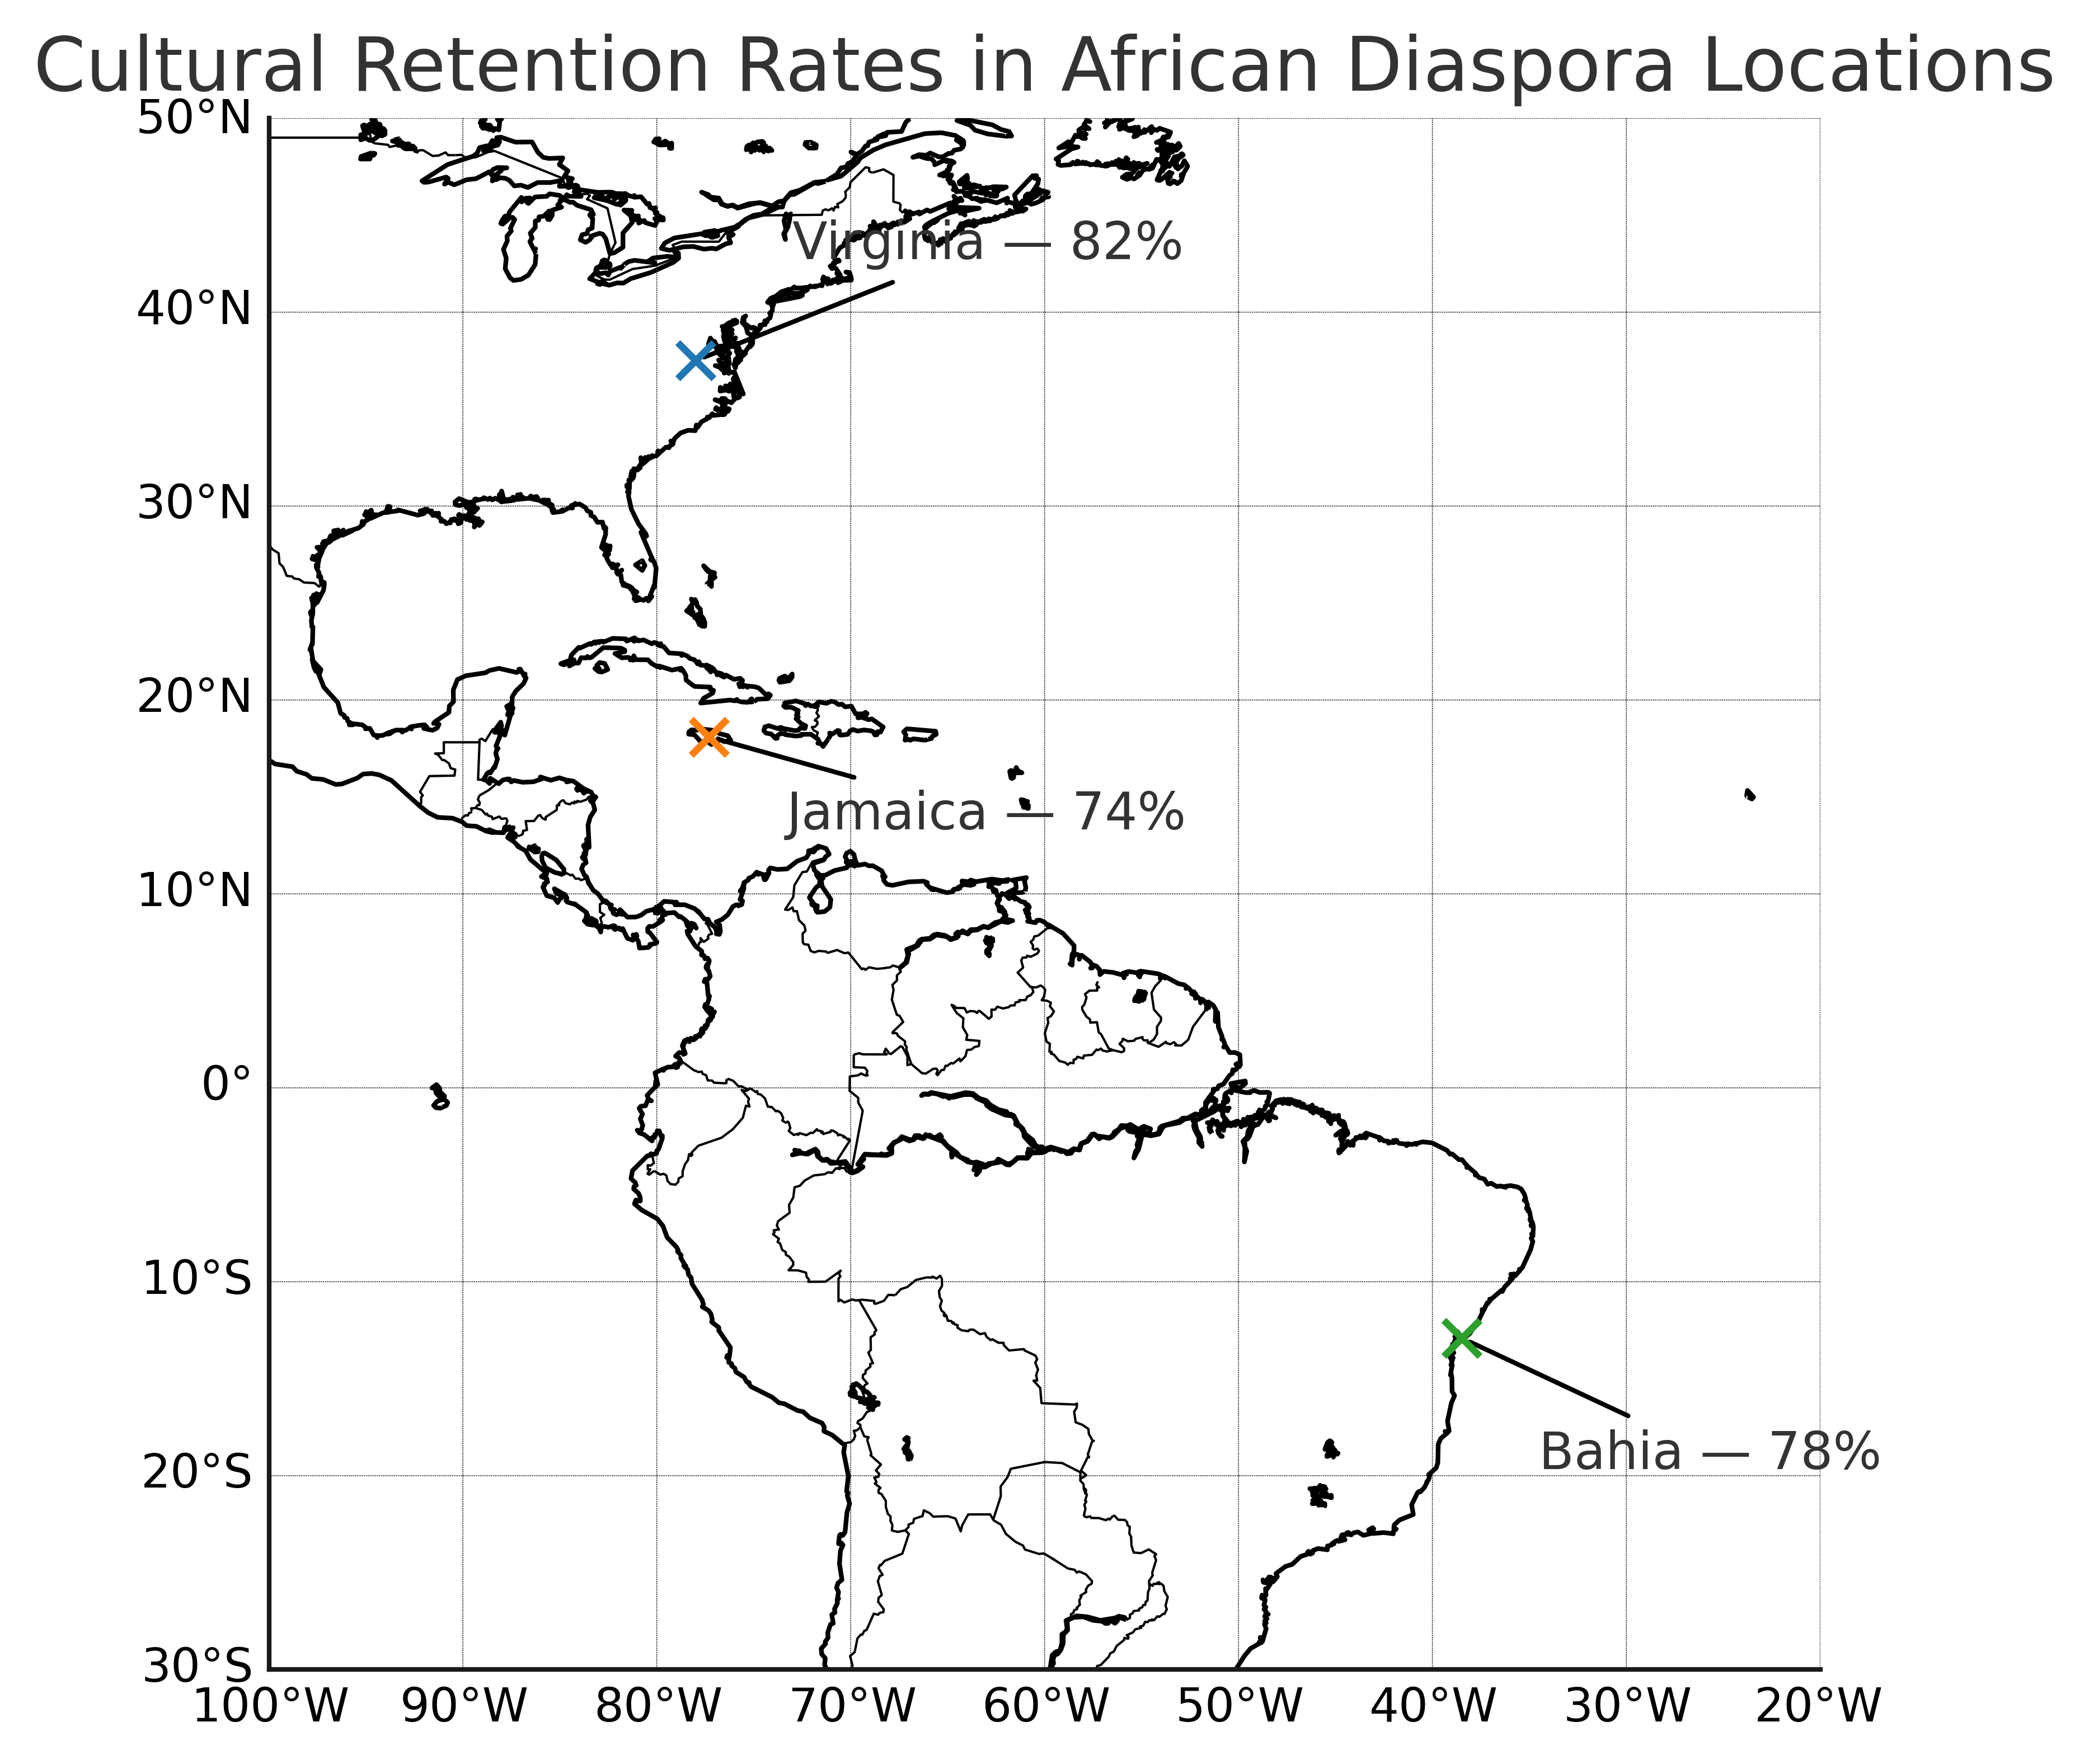
\includegraphics[width=0.85\linewidth]{cultural_retention_map.png}
  }{
    \fbox{\parbox[c][2in][c]{0.85\linewidth}{\centering
      Placeholder: cultural_retention_map.png not found}}
  }
  \caption{Map used for rapid verification of cultural retention rates.}
  \label{fig:retention-map}
\end{figure}

\FloatBarrier

% Print bibliography only if references.bib exists;
% If it exists but there are no explicit \cite commands in S1,
% \nocite{*} prevents the "empty bibliography / no citations" warnings.
\IfFileExists{references.bib}{
  \nocite{*}
  \printbibliography
}{}

\end{document}
